%presentation
\documentclass{beamer}

%impressions
%\documentclass[handout]{beamer}
%\usepackage{pgfpages}
%\pgfpagesuselayout{2 on 1}[a4paper,border shrink=5mm]
%\setbeameroption{notes on second screen}
%\pgfpagelayout{2 on 1}[a4paper, border, shrink=5mm]
% vue sur http://wwwtaketorg/spip/articlephp3?id_article=30...
\usepackage[T1]{fontenc}
\usepackage[frenchb]{babel}
\usepackage[utf8x]{inputenc} % Pour pouvoir taper les accents sans faire de combinaison
%\usepackage{arev}
%\usepackage{aeguill}
%mode code
\usepackage{listings}

%mode verbatim
\usepackage{moreverb}

%\usepackage[darktab]{beamerthemesidebar}
%\leftsidebar
%\usetheme{Hannover}
%\usetheme{Warsaw}
%\usetheme{PaloAlto}
\usetheme{JuanLesPins}
%\usetheme{Antibes}
%\usetheme{Shingara}
%\usetheme{Berlin}
%\usetheme{Oxygen}
\usepackage{thumbpdf}
\usepackage{wasysym}
\usepackage{ucs}
\usepackage{pgfarrows,pgfnodes,pgfautomata,pgfheaps,pgfshade}
\usepackage{verbatim}
\usepackage{color}

\AtBeginSection[]
{
  \begin{frame}<beamer>
    \tableofcontents[currentsection,currentsubsection]
  \end{frame}
}


\title{Ruby, Ruby on Rails et le déploiement sur serveur d'application}
\author{Cyril Mougel}

\logo{
\includegraphics[width=10mm]{rails.png}}

\begin{document}

\begin{frame}
    \titlepage
\end{frame}

\section{Le langage Ruby}

\begin{frame}
	\frametitle{L'historique}
	\begin{itemize}
		\item Créé en 1993 par Yukihiro Matsumoto dit \og{}Matz\fg{}
		\item Langage de scripting de haut niveau
		\item Plus qu'orienté objet: tout est objet
        \item Applique le principe de moindre surprise (POLS, \emph{principle of
                least surprise})
        \item Fonctionne sur les plateformes les plus populaires du marché (Linux, Windows,
                Mac)
	\end{itemize}
\end{frame}

\section{Les concepts de Ruby on Rails}


\begin{frame}
    \frametitle{Le framework Ruby on Rails}
    \begin{itemize}
        \item Créé par David Heinemeier Hansson dit \og{}DHH\fg{}
        \item Extrait de l'application BaseCamp de 37signals
        \item Première \emph{public release} en 2004 
    \end{itemize}
\end{frame}

\begin{frame}
    \frametitle{Pourquoi Rails en Ruby ?}
    \begin{itemize}
        \item Multi-plateformes
        \item Fortes facilités d'introspection et de réflexion
            \begin{itemize}
                \item User.find\_by\_firstname\_and\_lastname 'David', 'Hanson'
                \item has\_many :galleries
            \end{itemize}
    \end{itemize}
\end{frame}

\begin{frame}
    \frametitle{Le concept de Ruby on Rails}
    \begin{itemize}
        \item Ruby on Rails est conçu par des développeurs, pour des développeurs
        \item Un cadre de travail minimal et complet pour le développement Web
        \item \emph{Convention over Configuration}
        \item \emph{Don't Repeat Yourself} (DRY)
        \item \emph{Say what you do, Do what you say}
        \item Un seul et unique langage pour tout faire
    \end{itemize}
\end{frame}

\begin{frame}
    \frametitle{Rails est MVC}
    \begin{itemize}
        \item Model : ActiveRecord
        \item View : ActionView
        \item Controller : ActionController
    \end{itemize}
\end{frame}

\begin{frame}
    \frametitle{Chaque chose à sa place}
    Chaque dossier correspond à quelque chose et a son utilité
            propre
    \begin{columns}
        \begin{column}[l]{4cm}
            \begin{figure}
                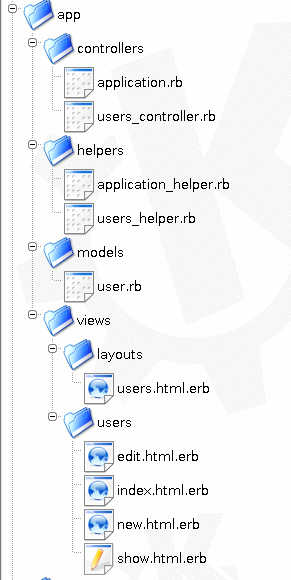
\includegraphics[width=30mm]{FS_1.png}
            \end{figure}
        \end{column}
        \begin{column}[r]{4cm}
            \begin{figure}
                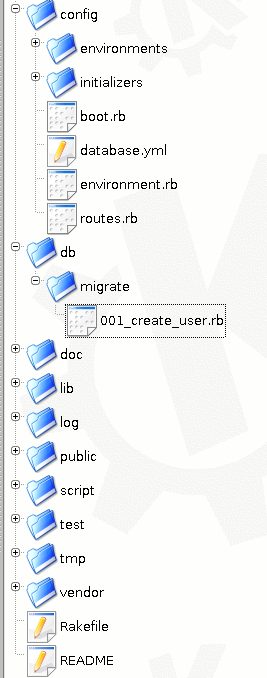
\includegraphics[width=25mm]{FS_2.png}
            \end{figure}
        \end{column}
    \end{columns}
\end{frame}

\section{Composant Model de Ruby on Rails}

\begin{frame}
    \frametitle{Gestion de la Base de données}
    \begin{itemize}
        \item Système de gestion de migration (ActiveRecord::Migration)
        \item Utilisation du pattern ActiveRecord
        \item Génération de nombreuses méthodes utilitaires à la volée
    \end{itemize}
\end{frame}

\begin{frame}
    \frametitle{Migration de Base de donnée}
    \begin{itemize}
        \item Gestion incrémentale des fichiers de migrations
        \item Retour avant/arrière au sein des migrations
        \item Utilisation de méthodes Ruby au lieu de requêtes SQL pur
    \end{itemize}
\end{frame}
\begin{frame}
    \frametitle{Exemple de Migration}

    Un exemple de fichier de migration :


    \begin{center}
        \lstinputlisting[language=Ruby,basicstyle=\scriptsize,
        numbers=left]{066_fix_profiles.rb}
    \end{center}
\end{frame}

\begin{frame}
    \frametitle{La classe Mapping}
    Exemple de fichier qui mappe la table Projects qui possèdent 6 champs~:
   
    \begin{columns}
        \begin{column}[l]{3cm}
            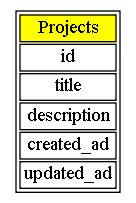
\includegraphics[width=20mm]{project.png}
        \end{column}
        
        \begin{column}[r]{10cm}
            \begin{block}{Code de la classe de Mapping}
              \lstinputlisting[language=Ruby,numbers=left,basicstyle=\scriptsize]{project.rb}        
            \end{block}
            \begin{block}{Exemple d'utilisation de la classe de mapping}
              \lstinputlisting[language=Ruby,numbers=left,basicstyle=\scriptsize]{project_use.rb}        
            \end{block}
        \end{column}
    \end{columns}

\end{frame}

\begin{frame}
    \frametitle{les méthodes \emph{static} accessibles pour la classe Project}
    Et bien-sûr toutes les méthodes accessibles en \emph{static}~:
    \tiny{}
    \begin{columns}
        \begin{column}[l]{5cm}
            \begin{itemize}
                \item Project.find :all
                \item Project.find\_by\_title 'EDF Entreprise'
                \item Project.find\_by\_description 'un site'
                \item Project.find\_by\_title\_and\_description 'EDF', 'site'
            \end{itemize}
        \end{column}

        \begin{column}[r]{6cm}
            \begin{itemize}
                \item Project.count :all
                \item Project.count\_by\_title 'EDF Entreprise'
                \item Project.count\_by\_description 'un site'
                \item Project.count\_by\_title\_and\_description 'EDF', 'site'
            \end{itemize}
        \end{column}
    \end{columns}
    \normalsize{}
    etc\ldots
\end{frame}

\begin{frame}
    \frametitle{le système de validation du modèle}
    Multiples systèmes de validation pour empêcher l'enregistrement en base de
    données d'informations erronées
    \scriptsize{}
    \begin{columns}
        \begin{column}[l]{5cm}
            \lstinputlisting[language=Ruby,numbers=left,basicstyle=\tiny]{project2.rb}
        \end{column}

        \begin{column}[r]{5cm}
            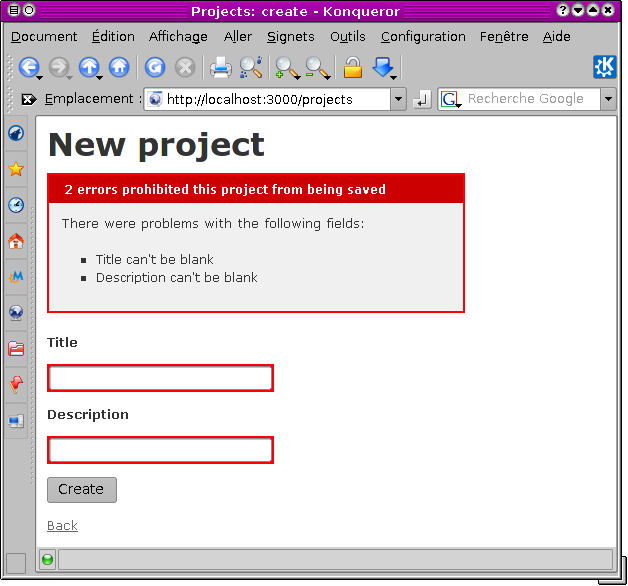
\includegraphics[width=60mm]{error_screenshot.png}
        \end{column}
    \end{columns}
\end{frame}

\begin{frame}
    \frametitle{Les associations}
    \begin{center}
        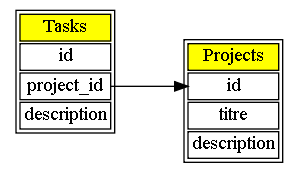
\includegraphics[width=40mm]{project_task.png}
        \lstinputlisting[language=Ruby,numbers=left,basicstyle=\scriptsize]{project3.rb}
    \end{center}
\end{frame}


\section{Composant Controller de Ruby on Rails}

\begin{frame}
    \frametitle{1 méthode, 1 URL}
    \begin{itemize}
        \item Url implicite à partir du nom de controller et du nom de la
        méthode
        \item Utilisation de routes nommées
        \item Définition implicite du fichier de Vue
    \end{itemize}
\end{frame}

\begin{frame}
    \frametitle{RESTFULL}

    \begin{itemize}
        \item REST (Representational State Transfer)
        \item Basé sur les 4 verbes HTTP~:
            \begin{itemize}
                \item POST (create)
                \item GET (show)
                \item PUT (update)
                \item DELETE (delete)
            \end{itemize}
        \item Utilisation des verbes simples avec URL correspondant
        \item Facilité de création d'une API
    \end{itemize}
\end{frame}

\begin{frame}
    \frametitle{Exemple de controller}
    \lstinputlisting[language=Ruby,numbers=left,basicstyle=\scriptsize]{project_controller.rb}
\end{frame}

\section{Composant de Vue de Ruby On Rails}

\begin{frame}
    \frametitle{Les helpers}

    \begin{itemize}
        \item 1 helper par controller par défaut
        \item réutilisation des manipulations de vues
        \item de nombreuses méthodes existantes dans l'API
    \end{itemize}
\end{frame}

\begin{frame}
    \frametitle{ActionView}
    \begin{block}{app/views/project/list.html.erb}
        \lstinputlisting[language=Ruby,numbers=left,basicstyle=\tiny,showspaces=false,showstringspaces=false]{list.html.erb}
    \end{block}
    \begin{block}{app/views/project/show.html.erb}
        \lstinputlisting[language=Ruby,numbers=left,basicstyle=\tiny,showspaces=false,showstringspaces=false]{show.html.erb}
    \end{block}
    \begin{block}{app/views/task/\_task.html.erb}
        \lstinputlisting[language=Ruby,numbers=left,basicstyle=\tiny,showspaces=false,showstringspaces=false]{_task.html.erb}
    \end{block}
\end{frame}


\section{Les tests}

\begin{frame}
    \frametitle{Les tests unitaires}
    \begin{itemize}
        \item Dans le dossier /test/units
        \item Test sur les classes models
        \item Facilité de créer des jeux de tests
        \item Base de données indépendante
        \item Réinjection automatique des données à chaque test
    \end{itemize}
\end{frame}

\begin{frame}
    \frametitle{Les tests fonctionnels}
    \begin{itemize}
        \item Dans le dossier /test/functionals
        \item Test sur les controllers
        \item Même système d'injection des jeux de données
        \item Assertion spécifique avec vérification du DOM
    \end{itemize}
\end{frame}

\section{Outils de développement}

\begin{frame}
    \frametitle{Les environnements de développement}
    \begin{itemize}
        \item Netbeans depuis la version 6.0 
        \item Aptana, plugin d'eclipse
        \item Ruby In Steel, add-on de Microsoft Visual Studio
        \item Vim/Emacs
    \end{itemize}
\end{frame}

\begin{frame}
    \frametitle{Outils d'aide au développement}
    \begin{itemize}
        \item Shell Interactif, irb
        \item Debugger
        \item Profiler
        \item Couverture de code
    \end{itemize}
\end{frame}

\section{Java, Jruby et Ruby On Rails}

\begin{frame}
    \frametitle{JRuby implémentation Java de Ruby}
    \begin{itemize}
        \item JRuby 1.0 sortie en Juin 2007, 1.1 en Avril 2008
        \item Entièrement compatible avec Ruby 1.8.6
        \item Intégration avec toute bibliothèque Java existante
    \end{itemize}
\end{frame}

\begin{frame}
    \frametitle{JRuby on Rails}
    \begin{itemize}
        \item Depuis JRuby 1.0.2, possibilité de faire tourner Ruby On Rails
        \item Possibilité de générer un WAR avec le plugin Goldspike
        \item War généré utilisable dans un serveur d'application
    \end{itemize}
\end{frame}

\begin{frame}
    \begin{center}
    \huge{}
    demo
    \end{center}
\end{frame}

\end{document}
